% Figure 7: Cost Comparison Across Usage Scenarios
\begin{figure}[htbp]
\centering
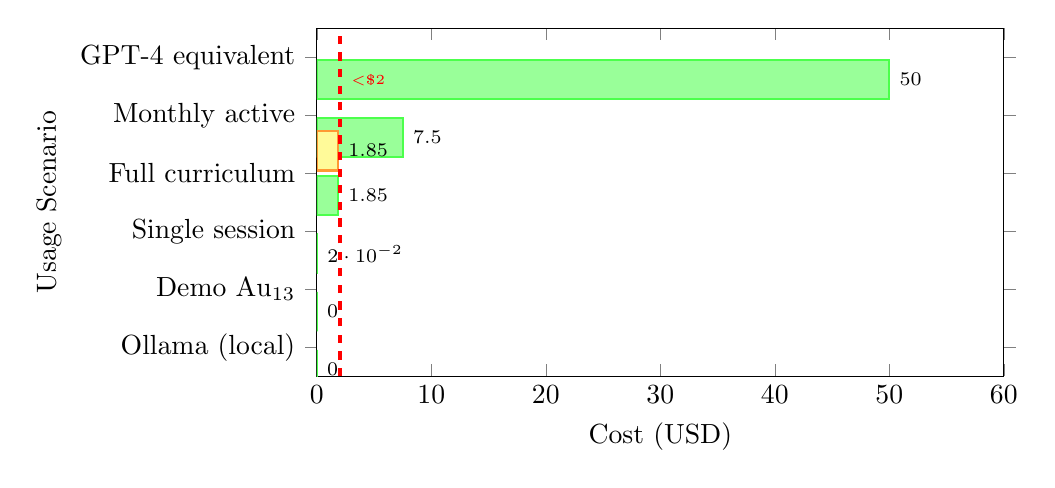
\begin{tikzpicture}
\begin{axis}[
    xbar,
    width=0.85\textwidth,
    height=6cm,
    xlabel={Cost (USD)},
    ylabel={Usage Scenario},
    ytick={0,1,2,3,4,5},
    yticklabels={
        Ollama (local),
        Demo Au$_{13}$,
        Single session,
        Full curriculum,
        Monthly active,
        GPT-4 equivalent
    },
    ymin=-0.5,
    ymax=5.5,
    xmin=0,
    xmax=60,
    nodes near coords,
    nodes near coords align={horizontal},
    every node near coord/.append style={font=\scriptsize},
    bar width=0.5cm,
]

% Cost bars with explicit colors
\addplot[fill=green!40, draw=green!70, thick] coordinates {
    (0, 0)
    (0, 1)
    (0.02, 2)
    (1.85, 3)
    (7.5, 4)
    (50, 5)
};

% Highlight <$2 threshold
\addplot[fill=yellow!40, draw=orange!80, thick] coordinates {
    (1.85, 3)
};

% Add reference lines
\draw[dashed, red, ultra thick] (axis cs:2,-0.5) -- (axis cs:2,5.5) 
    node[pos=0.85, right, font=\tiny, text=red] {\textless\$2};

\end{axis}
\end{tikzpicture}
\caption{Cost comparison across usage scenarios. The framework provides three cost tiers: (1) \textbf{Zero-cost} — Demo Au$_{13}$ pipeline and Ollama local inference require no API access, (2) \textbf{Ultra-low-cost} — Complete 25-notebook curriculum execution via OpenRouter costs <\$2, enabling genuine accessibility, and (3) \textbf{Production} — Monthly active researcher costs <\$10, still 5× cheaper than GPT-4 baseline. The dual-path architecture addresses reproducibility without excluding resource-constrained institutions.}
\label{fig:cost_comparison}
\end{figure}
